% ----------------- Documento ----------------- %
% Se define el tipo de documento (en este caso un artículo), en hoja A4 con tamaño de fuente de 11pt, escrito en castellano, e indicando que el documento tendrá páginas distintas a izquierda y derecha ("twoside"):
\documentclass[a4paper, 11pt, spanish, twoside]{article}
% Los demás tipos de documentos así como sus características y opciones pueden consultarse en: https://en.wikibooks.org/wiki/LaTeX/Document_Structure#Document_classes
% ---------------------------------------------- %


%%%%%%%%%%%%%%%%% - PREÁMBULO - %%%%%%%%%%%%%%%%% 

% ------------------ Página -------------------- %
% Se define el tamaño de las páginas, indicando el tamaño de los márgenes superior e inferior ("top" y "bottom"), e izquierdo y derecho ("left" y "right"):
\usepackage[top=2.5cm,bottom=2.5cm,left=2.5cm,right=2.5cm]{geometry}
% Se inserta el comando \raggedbottom para evitar que LaTeX rellene con espacios en blanco aquellas páginas que no alberguen suficiente contenido como para rellenarlas de forma "natural":
\raggedbottom 
% ---------------------------------------------- %


% ------------- Paquetes generales ------------- %
% Se importan distintos paquetes de propósito general:
\usepackage[utf8]{inputenc}
\usepackage[spanish]{babel}
\usepackage{float}
\usepackage{caption}
% ---------------------------------------------- %


% ------------ Paquetes específicos ------------ %
% Se importan distintos paquetes que será utilizados en momentos concretos del documento: 
\usepackage{pdfpages} % Para insertar la portada en formato PDF.
\usepackage{amssymb} % Para símbolos matemáticos.
\usepackage{bm} % Para negrita en símbolos matemáticos.
\usepackage{amsmath} % Para el entorno "split".
\usepackage[hidelinks]{hyperref} % Para urls.
\usepackage{longtable} % Para tablas largas.
\usepackage{graphicx} % Para insertar imágenes.
\usepackage{wrapfig} % Para posicionar imágenes alrededor del texto.
\usepackage{fontawesome5} % Para utilizar iconos de "fontawesome".
\usepackage{pdflscape}  % Para colocar páginas en formato apaisado.
\usepackage[T1]{fontenc}
\usepackage{textcomp}
\usepackage{lmodern} % Soluciona el problema de la mala resolución
\usepackage{url}

% ---------------------------------------------- %


% ---------------- Numeración ------------------ %
\counterwithin{table}{section} % Se numeran las tablas con respecto al capítulo en el que se encuentran.
\counterwithin{figure}{section} % Se numeran las figuras con respecto al capítulo en el que se encuentran.
\counterwithin{equation}{section} % Se numeran las ecuaciones con respecto al capítulo en el que se encuentran.
% ---------------------------------------------- %


% ------------- Página en blanco ----------------%
% Se define un comando (\blankpage) para insertar una página totalmente en blanco (sin número de página, encabezado y pie de página):
\usepackage{afterpage}
\newcommand\blankpage{%
    \null
    \thispagestyle{empty}%
    \newpage}
% ---------------------------------------------- %    


% ----------- Formato de los párrafos -----------%
% Se define el formato de los párrafos:
\setlength{\parindent}{0pt} % Se elimina la sangría en comienzo de párrafo (0pt).
\setlength{\parskip}{1em} % Se define el espacio entre dos párrafos (1em).
% ---------------------------------------------- %    

% -------------- Título adicional -------------- %
% Se añade una profundidad adicional a los títulos (profundidad 4):
\usepackage{titlesec}
\setcounter{secnumdepth}{4} % Se fija en 4 la profundidad de numeración de títulos.
\setcounter{tocdepth}{4} % Se fija en 4 la profundidad de títulos incluidos en el índice.
% Se modifica el formato de \paragraph (título de profundidad 4) para adaptarlo al formato del resto de títulos:
\titleformat{\paragraph}
{\normalfont\normalsize\bfseries}{\theparagraph}{1em}{}
\titlespacing*{\paragraph}
{0pt}{3.25ex plus 1ex minus .2ex}{1.5ex plus .2ex} 
% ---------------------------------------------- %    


% --------- Encabezado y pie de página -------- %
% El encabezado y pie de página forman parte del paquete fancyhdr:
\usepackage{fancyhdr}
\fancyhf{}
\pagestyle{fancy}

% Para solucionar error "headheight is too small":%
\setlength{\headheight}{14.6pt}
\addtolength{\topmargin}{-0.6pt}

% Se ajusta el tamaño de fuente para el encabezado y pie de página (9pt)
\fancyhf{\fontsize{2}{14}\selectfont}

% Contenido del encabezado (\fancyhead):
\fancyhead[RO]{Simulación de operación de una central nuclear} % Texto que se coloca en el encabezado de las páginas impares (O -> 'Odd', o impar) a la izquierda (R -> 'Odd')
\fancyhead[LE]{\nouppercase{\rightmark}} % Texto que se coloca en el encabezado de las páginas pares (E -> 'Even', o par) a la izquierda (L -> 'Left'). \rightmark se utiliza para insertar automáticamente el título de la sección correspondiente, y \nouppercase para que no aparezca todo en mayúsculas (formato por defecto de \rightmark).

% Contenido del pie de página (\fancyfoot):
\fancyfoot[RE]{Escuela  Técnica  Superior  de  Ingenieros  Industriales  (UPM)} % Texto que se coloca en el pie de página de las páginas pares (E -> 'Even', o par) a la derecha (R -> 'Right')
\fancyfoot[LO]{Antonio Dies Beneytez} % Texto que se coloca en el pie de página de las páginas impares (O -> 'Odd', o impar) a la izquierda (L -> 'Left')
\fancyfoot[LE,RO]{\thepage} % El número de página (\thepage) se coloca a la izquierda en las páginas pares y a la derecha en las impares.

% Se indica que sólo se quiere incorporar en \rightmark (utilizado más arriba) el título de la sección (y no de las subsecciones, subsubsecciones, etc.):
\renewcommand{\sectionmark}[1]{\markright{\thesection. #1}}
\renewcommand{\subsectionmark}[1]{}

% Formato de la línea de separación horizontal:
\renewcommand{\headrulewidth}{0.5pt} % Ancho de la línea del encabezado.
\renewcommand{\footrulewidth}{0.5pt} % Ancho de la línea del pie de página.
% ---------------------------------------------- % 


% ----------- Fragmentos de código ------------- %
% El paquete utilizado para insertar fragmentos de código en el documento es listings. En el presente bloque del preámbulo se definen ciertos parámetros de listings con el objetivo de adaptar dicho paquete a código escrito en Python.

\usepackage{listings} % Paquete para insertar código. 
\usepackage{xcolor} % Paquete para definir colores.

% Se definen los distintos colores que se utilizan para resaltar ciertos elementos del código:
\definecolor{codegreen}{rgb}{0.04314,0.6745,0.07843} % Verde.
\definecolor{codegray}{rgb}{0.5,0.5,0.5} % Gris.
\definecolor{codered}{rgb}{0.5373,0.02745,0.06275} % Rojo.
\definecolor{codeblue}{rgb}{0.071,0.0258,0.9882} % Azul.
\definecolor{codepurple}{rgb}{0.6,0.02745,0.5961} % Morado.

% Se define el color de fondo:
\definecolor{backcolour}{rgb}{0.95,0.95,0.92} % Gris oscuro.

% Se define el valor de ciertos parámetros de listings para adaptar dicho paquete a código escrito en Python:
\lstdefinestyle{mystyle}{
    % - General:
    language=Python, % Lenguaje de programación.
    basicstyle=\ttfamily\footnotesize, % Tipografía y tamaño de fuente.
    % - Colores de los distintos elementos del código:
    backgroundcolor=\color{backcolour}, % Color de fondo.  
    commentstyle=\color{codegray}, % Color de los comentarios.
    keywordstyle=\color{codeblue}, % Color de las palabras clave por defecto.
    stringstyle=\color{codegreen}, % Color de los "string"
    % - Palabras clave:
    deletekeywords={print}, % Se elimina "print" del conjunto de palabras clave para posteriormente asignarle el color morado.
    keywordstyle={[2]\ttfamily\color{codeblue}},
    keywords=[2]{as}, % Se añaden las palabras clave de color azul.
    keywordstyle={[3]\ttfamily\color{codepurple}},
    keywords=[3]{True, False, ttk, list, None, dict, zip, range, len, print, float, sum}, % Se añaden las palabras clave de color morado.
    keywordstyle={[4]\bfseries\ttfamily},
    keywords=[4]{_read_excel}, % Se añaden las palabras clave en negrita.
    emph={MyClass,__init__}, % Se añaden las palabras clave enfatizadas.   
    % - Números de línea:
    numberstyle=\tiny\color{codegray}, % Tamaño de fuente y color de los números de línea.
    numbers=left, % Se colocan los números de línea en el lado izquierdo.                 
    numbersep=5pt, % Separación horizontal de los números de línea.
    % - Saltos a la línea, espacios, indentación:
    breaklines=true, % Permitir saltos a la línea. 
    breakatwhitespace=true, % Saltar a la línea únicamente al encontrar espacios.
    postbreak = \mbox{{$\hookrightarrow$}\space}, % Se añade una flecha al cambiar de línea.
    showspaces=false, % No mostrar los espacios. 
    showstringspaces=false, % No mostrar los espacios en los "string".
    keepspaces=true, % Mantener los espacios presentes en el código. 
    tabsize=2, % Tamaño de indentación.
    % - Título:
    captionpos=b % Posición del título del fragmento de código (b=bottom - abajo).
} 
\lstset{style=mystyle} % Se asocia el estilo de listings al estilo que acaba de definirse ("mystyle")

% Se realizan una serie de operaciones complementarias con el paquete listings (su comprensión no es necesaria para manejar dicho paquete):
\makeatletter
\def\lst@OpLiteratekey#1\@nil@{\let\lst@ifxopliterate\lst@if
                             \def\lst@opliterate{#1}}
\lst@Key{opliterate}{}{\@ifstar{\lst@true \lst@OpLiteratekey}
                             {\lst@false\lst@OpLiteratekey}#1\@nil@}
\lst@AddToHook{SelectCharTable}
    {\ifx\lst@opliterate\@empty\else
         \expandafter\lst@OpLiterate\lst@opliterate{}\relax\z@
     \fi}
\def\lst@OpLiterate#1#2#3{%
    \ifx\relax#2\@empty\else
        \lst@CArgX #1\relax\lst@CDef
            {}
            {\let\lst@next\@empty
             \lst@ifxopliterate
                \lst@ifmode \let\lst@next\lst@CArgEmpty \fi
             \fi
             \ifx\lst@next\@empty
                 \ifx\lst@OutputBox\@gobble\else
                   \lst@XPrintToken \let\lst@scanmode\lst@scan@m
                   \lst@token{#2}\lst@length#3\relax
                   \lst@XPrintToken
                 \fi
                 \let\lst@next\lst@CArgEmptyGobble
             \fi
             \lst@next}%
            \@empty
        \expandafter\lst@OpLiterate
    \fi}

\lstset{ 
    literate={á}{{\'a}}1 {é}{{\'e}}1 {í}{{\'i}}1 {ó}{{\'o}}1 {ú}{{\'u}}1
  {Á}{{\'A}}1 {É}{{\'E}}1 {Í}{{\'I}}1 {Ó}{{\'O}}1 {Ú}{{\'U}}1
  {à}{{\`a}}1 {è}{{\`e}}1 {ì}{{\`i}}1 {ò}{{\`o}}1 {ù}{{\`u}}1
  {À}{{\`A}}1 {È}{{\'E}}1 {Ì}{{\`I}}1 {Ò}{{\`O}}1 {Ù}{{\`U}}1
  {ä}{{\"a}}1 {ë}{{\"e}}1 {ï}{{\"i}}1 {ö}{{\"o}}1 {ü}{{\"u}}1
  {Ä}{{\"A}}1 {Ë}{{\"E}}1 {Ï}{{\"I}}1 {Ö}{{\"O}}1 {Ü}{{\"U}}1
  {â}{{\^a}}1 {ê}{{\^e}}1 {î}{{\^i}}1 {ô}{{\^o}}1 {û}{{\^u}}1
  {Â}{{\^A}}1 {Ê}{{\^E}}1 {Î}{{\^I}}1 {Ô}{{\^O}}1 {Û}{{\^U}}1
  {Ã}{{\~A}}1 {ã}{{\~a}}1 {Õ}{{\~O}}1 {õ}{{\~o}}1
  {œ}{{\oe}}1 {Œ}{{\OE}}1 {æ}{{\ae}}1 {Æ}{{\AE}}1 {ß}{{\ss}}1
  {ű}{{\H{u}}}1 {Ű}{{\H{U}}}1 {ő}{{\H{o}}}1 {Ő}{{\H{O}}}1
  {ç}{{\c c}}1 {Ç}{{\c C}}1 {ø}{{\o}}1 {å}{{\r a}}1 {Å}{{\r A}}1
  {€}{{\euro}}1 {£}{{\pounds}}1 {«}{{\guillemotleft}}1
  {»}{{\guillemotright}}1 {ñ}{{\~n}}1 {Ñ}{{\~N}}1 {¿}{{?`}}1
  {º}{{\textordmasculine}}1}

\lstset{opliterate=
   *{0}{{{\color{codered}0}}}1 {1}{{{\color{codered}1}}}1 
   {2}{{{\color{codered}2}}}1 {3}{{{\color{codered}3}}}1 
   {4}{{{\color{codered}4}}}1 {5}{{{\color{codered}5}}}1 
   {6}{{{\color{codered}6}}}1 {7}{{{\color{codered}7}}}1 
   {8}{{{\color{codered}8}}}1 {9}{{{\color{codered}9}}}1}

\DeclareCaptionType{code}[Código][ÍNDICE DE CÓDIGOS] % Se define el entorno "Código" (de forma que al introducir un fragmento de código en el documento aparezca como: Código 1.1: ...), y la lista con los distintos códigos ("Índice de códigos").
\counterwithin{code}{section} % Se numeran los códigos con respecto al capítulo en el que se encuentran.
% ---------------------------------------------- % 


% --------------- Bibliografía ----------------- %
% El manejo de la bibliografía se realiza mediante el paquete biblatex:
\usepackage[backend=bibtex, style=authoryear, sorting=nyt, citestyle=authoryear, maxcitenames=2, maxbibnames=5, giveninits=true, uniquename=init]{biblatex} 

% Los distintos parámetros que aparecen en la línea anterior corresponden a las siguientes características de la bibliografía:
% - style: la manera en la que aparecen las referencias en la bibliografía. En este caso se opta por "authoryear", pero existen múltiples estilos posibles que se resumen en la siguiente guía: https://www.overleaf.com/learn/latex/biblatex_bibliography_styles.
% - sorting: orden en el que aparecen las distintas referencias en la bibliografía. En este caso se opta por ordenarlas en primer lugar por el apellido del primer autor, en segundo lugar por el año de publicación, y por último por el título de la publicación (nyt=name-year-title)
% - citestyle: elementos y orden de dichos elementos de una referencia al citarla en el documento. En este caso se escoge "authoryear" para que aparezca en primer lugar el apellido del autor (o de los autores) y en segundo lugar el año de publicación. Existe gran variedad de opciones en cuanto al parámetro citestyle que se resumen en: https://www.overleaf.com/learn/latex/biblatex_citation_styles.
% maxcitenames: máximo número de autores que aparecen al citar una referencia en el documento. Al escoger un valor de 2 para este parámetro se pueden dar los siguientes casos: un único autor -> (autor, año), dos autores -> (autor 1 y/e autor 2, año), tres o más autores -> (autor 1 et al., año).
% maxbibnames: parámetro idéntico al anterior pero para la bibliografía en lugar de las citas.
% giveinits y uniquename: para mostrar únicamente las iniciales de los nombres de los autores.

% Se importa el paquete csquotes para citar las referencias a lo largo del documento:
\usepackage{csquotes} 

% Se realizan una serie de operaciones para adaptar la bibliografía al estilo deseado (coma entre autor y año al citar una referencia, idioma castellano, etc.):
\DeclareNameAlias{sortname}{family-given}
\renewcommand*{\nameyeardelim}{\addcomma\space}
\setlength\bibitemsep{\baselineskip}
\DefineBibliographyStrings{spanish}{%
  andothers = {et\addabbrvspace al\adddot}
}

\makeatletter

\newrobustcmd*{\parentexttrack}[1]{%
  \begingroup
  \blx@blxinit
  \blx@setsfcodes
  \blx@bibopenparen#1\blx@bibcloseparen
  \endgroup}

\AtEveryCite{%
  \let\parentext=\parentexttrack%
  \let\bibopenparen=\bibopenbracket%
  \let\bibcloseparen=\bibclosebracket}

\makeatother

\addbibresource{content/sections/biblio.bib}

% --------------- Abreviaturas, unidades y acrónimos ----------------- %

\usepackage{glossaries}
\makenoidxglossaries

\newglossaryentry{simuladores}
{
    name=Simuladores,
    text={simuladores},
    description={Los simuladores son... Esto es un ejemplo para el glosario}
}

\newacronym{smr}{SMR}{Small Modular Reactors}
% ---------------------------------------------- % 


%%%%%%%%%%%% - INICIO DEL DOCUMENTO - %%%%%%%%%%%%

\begin{document} 


%%%%%%%%%%%%%%%%%%% - PORTADA - %%%%%%%%%%%%%%%%%%

% Se comienza una página nueva sin formato (sin número de página y sin encabezado/pie de página), ya que sólo incorpora la la portada:
\newpage
\thispagestyle{empty}

% La portada se inserta mediante el comando \includepdf seguido del archivo PDF correspondiente (que se ajusta automáticamente a las dimensiones de la página):
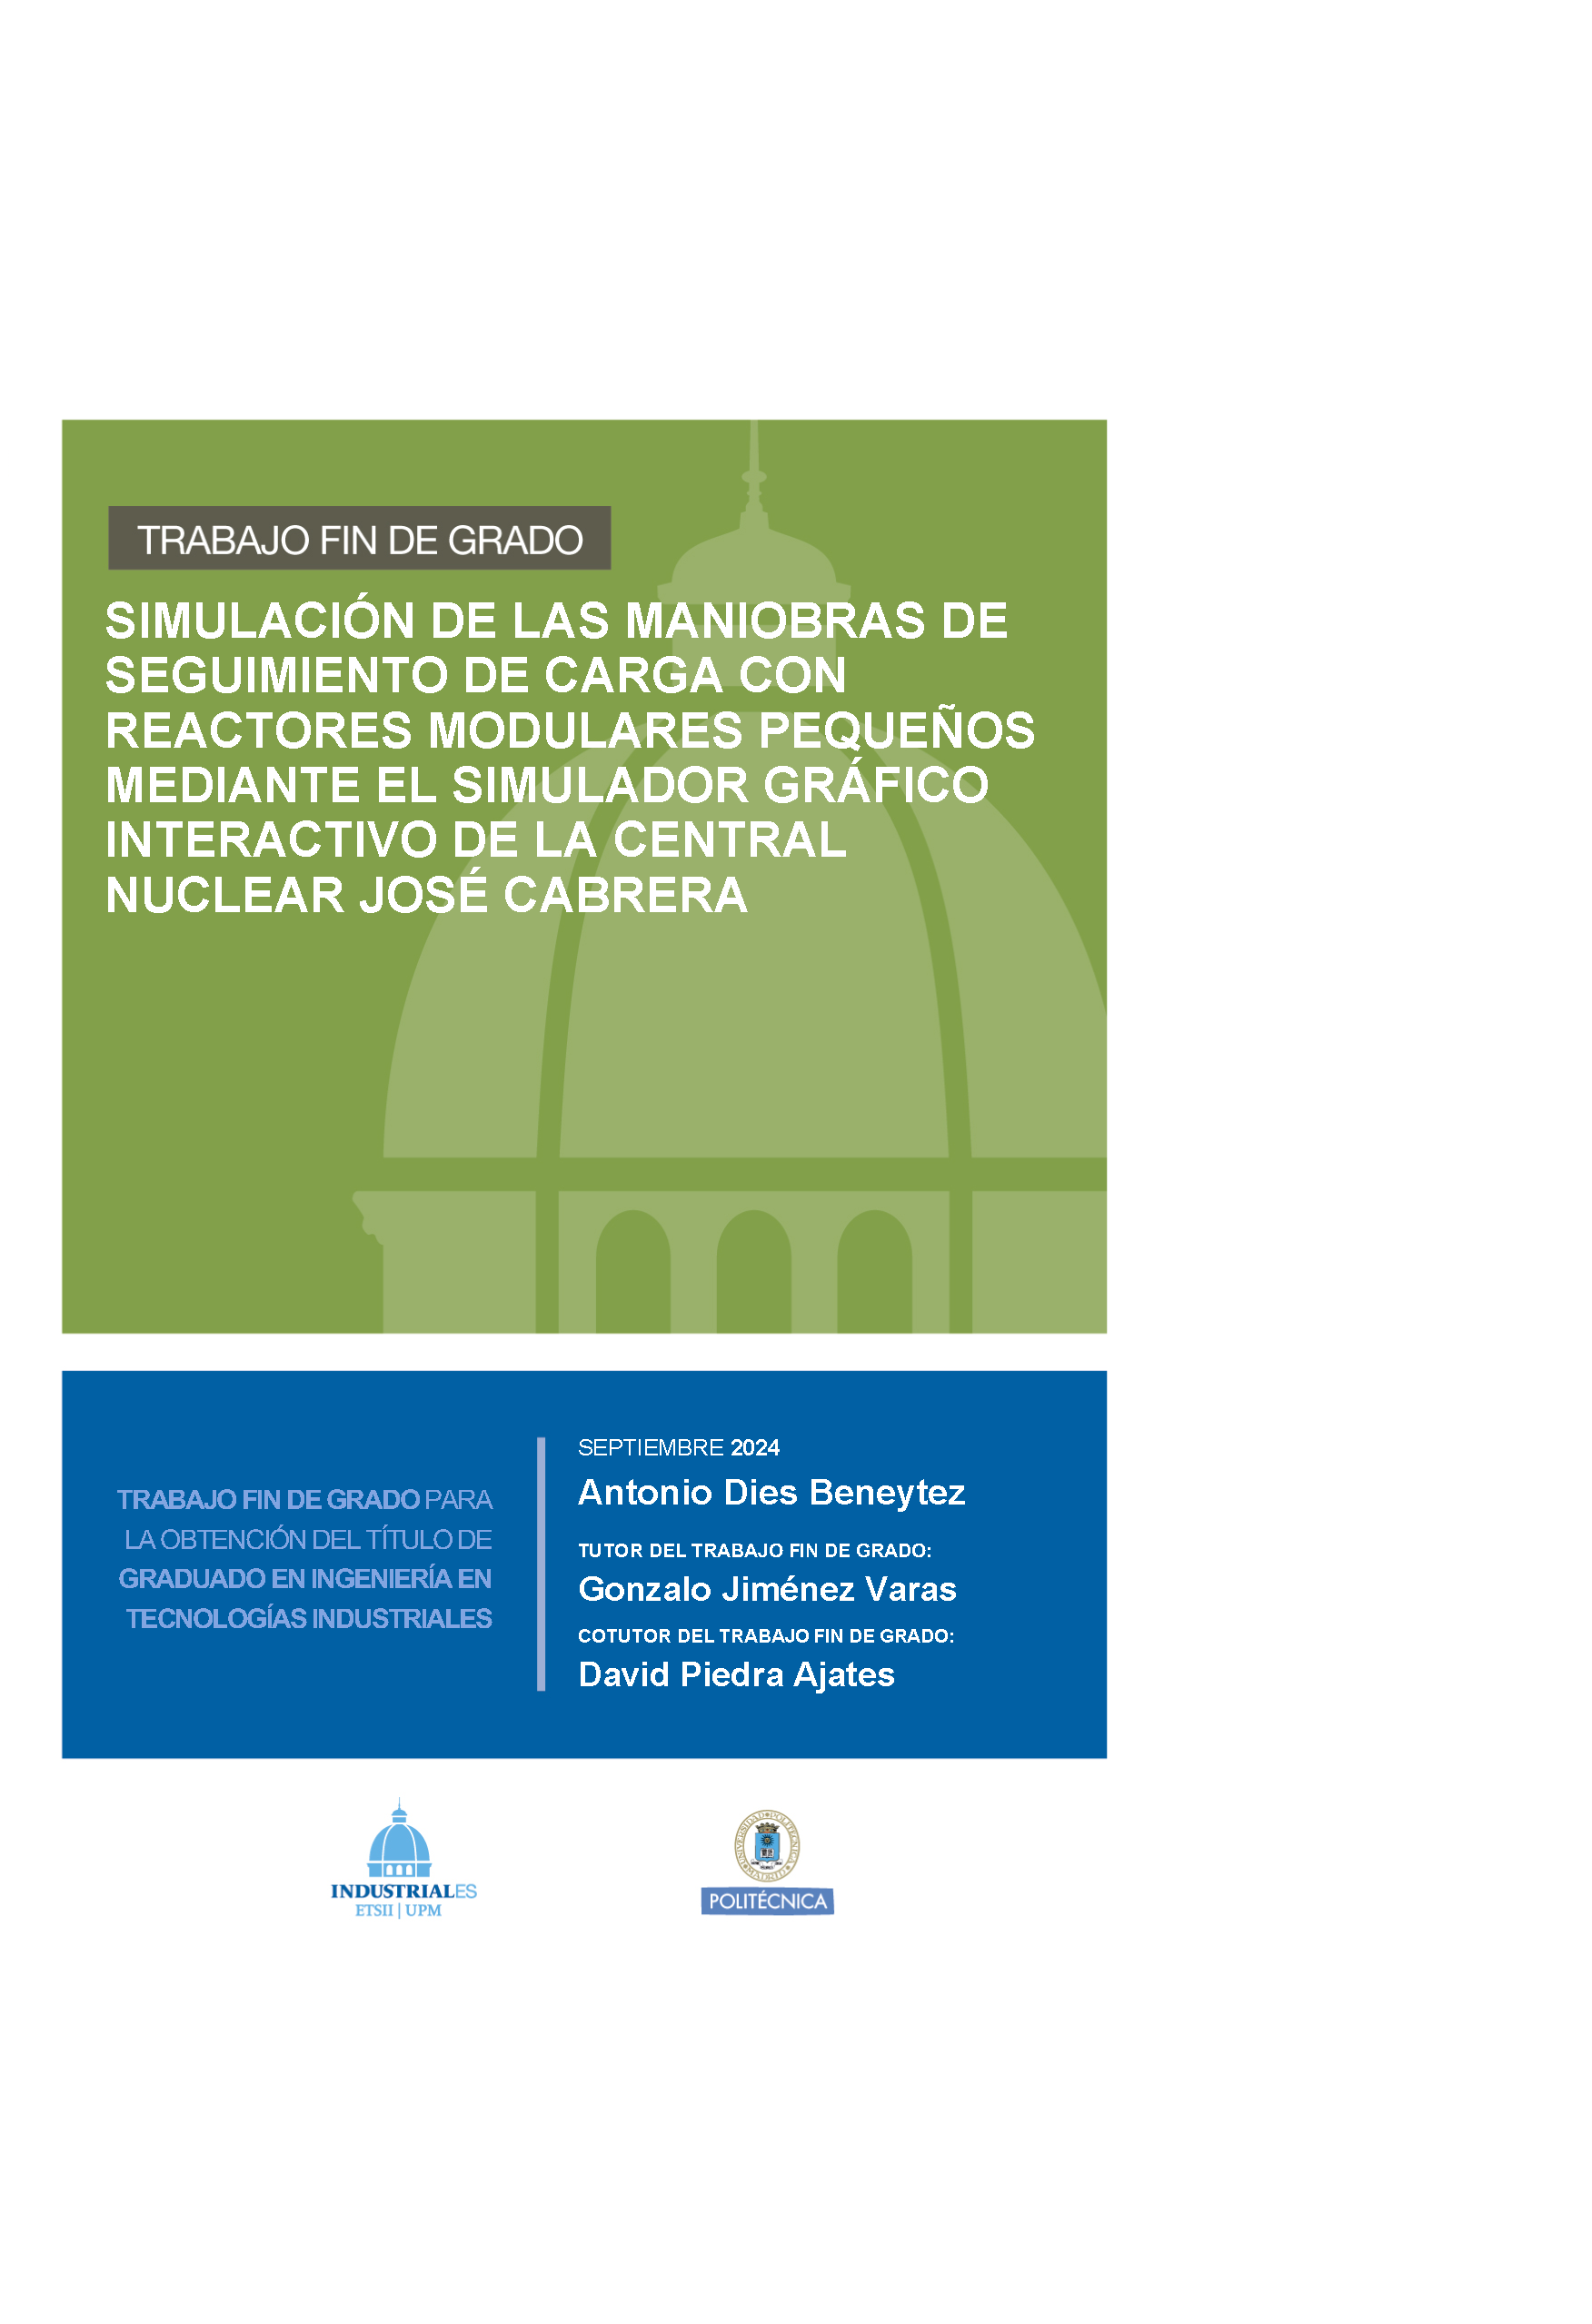
\includepdf{content/Portada_TFG_Antonio_Dies.pdf}

%%%%%%%%%%%%%%%%%%%%%%%%%%%%%%%%%%%%%%%%%%%%%%%%%%

% Las páginas anteriores al contenido del TFG/TFM (previas a la introducción) suelen numerarse de forma distinta a las del cuerpo del informe, en este caso en números romanos:
\pagenumbering{roman}


%%%%%%%%%%%%%$%%%%% - CITA - %%%%%%%%%%%%%%%%%%%%%
 
% Se comienza una página nueva sin formato (sin número de página y sin encabezado/pie de página), ya que sólo incorpora la cita:
\newpage
\thispagestyle{empty}

\begin{flushright} % Se alinea el texto en el lado derecho de la página.
\vspace*{5cm} % Se añade un espacio vertical de 5cm para situar la cita en ~1/3 de la página.

\textit{“La cita del trabajo iría aquí”} 

\medskip % Salto a la línea de tamaño medio (existen \smallskip, \medskip y \bigskip)
- El autor de la cita 

\end{flushright}

\afterpage{\blankpage} % Se añade una página en blanco después de la cita.


%%%%%%%%%%%%% - AGRADECIMIENTOS - %%%%%%%%%%%%%%%%

% Se comienza una página nueva con formato plano (sin encabezado/pie de página pero con número de página):
\newpage
\thispagestyle{plain}

\section*{AGRADECIMIENTOS} % Se añade un asterisco a \section para que el título no esté numerado.
\addcontentsline{toc}{section}{AGRADECIMIENTOS} % Al utilizar \section* se ha de añadir manualmente el apartado al índice (Table Of Contents, TOC).

Agradezco a \dots

Gracias a \dots

A \dots \ por \dots

\afterpage{\blankpage} % Se añade una página en blanco después de los agradecimientos.


%%%%%%%%%%%%%% - RESUMEN - %%%%%%%%%%%%%

\newpage
\section*{RESUMEN} % Se añade un asterisco a \section para que el título no esté numerado.
\markright{RESUMEN} % Al utilizar \section* se ha de añadir manualmente el título del apartado al encabezado.
\addcontentsline{toc}{section}{RESUMEN} % Al utilizar \section* se ha de añadir manualmente el apartado al índice (Table Of Contents, TOC).

Este documento constituye una guía (que sirve a su vez de plantilla) para la elaboración de informes de TFG o TFM en \LaTeX. No pretende abarcar todas y cada una de las funcionalidades que ofrece \LaTeX \ (¡las posibilidades son prácticamente infinitas!) pero sí tratar los aspectos fundamentales para la elaboración de un documento utilizando esta indispensable herramienta. Además de los elementos básicos de cualquier informe (índice, tablas, ecuaciones, bibliografía, etc.), esta guía incluye ``tutoriales'' y plantillas para algunos de los elementos presentes en todo (o casi todo) informe de TFG o TFM (como son el diagrama de Gantt o la EDP). 

\textbf{Nota:} se ha tratado de explicar con detalle la mayor parte de elementos presentes en el documento, ya sea por medio de los capítulos y apartados que lo conforman o mediante explicaciones bajo la forma de comentarios en el código \LaTeX. Es especialmente importante examinar con atención el preámbulo de dicho código, ya que en él se llevan a cabo muchas de las operaciones esenciales que dan forma al documento.

\afterpage{\blankpage} % Se añade una página en blanco después del resumen.


%%%%%%%%%%%%%%%%%%% - ÍNDICE - %%%%%%%%%%%%%%%%%%%

\newpage

\renewcommand*\contentsname{ÍNDICE} % Se modifica el nombre por defecto de la "Table Of Contents" (tabla de contenidos, índice) para pasar a llamarla "ÍNDICE".

\tableofcontents % Se genera el índice de contenidos del documento que incorpora todos los títulos de \section, \subsection y \subsubsection (y también \paragraph, ver capítulo 1), así como los títulos añadidos con \addcontentsline (como el resumen ejecutivo, por ejemplo).

\afterpage{\blankpage} % Se añade una página en blanco después del índice.


%%%%%%%%%%%%%%%%%%%%%%%%%%%%%%%%%%%%%%%%%%%%%%%%%%

% Se inicia una nueva página, y se restablece la numeración de las páginas, utilizando esta vez el sistema de numeración estándar (1, 2, 3, 4, ...)
\newpage
\pagenumbering{arabic}

%%%%%%%%%%%%%% - CONTENIDO - %%%%%%%%%%%%%%

\section{INTRODUCCIÓN} \label{sec:introduccion}

\subsection{Justificación}

Actualmente, el mundo atraviesa una crisis energética global desencadenada en el año 2021 principalmente por la recuperación económica tras la pandemia y agravada tras la invasión rusa de Ucrania en febrero de 2022. El precio del gas natural alcanzó máximos históricos, aumentando consecuentemente en muchos casos el coste de la electricidad en general. Familias, empresas e industrias se han visto gravemente afectadas, llevando a diversos países en camino de una fuerte recesión económica. Consecuentemente, la reducción de los costes energéticos se convierte en una de las principales prioridades de empresas y ciudadanos, y la independencia energética, la
garantía de suministro y la lucha contra el cambio climático adquieren una gran importancia en el debate público de gran cantidad de países (\cite{crisis_energetica_iea}). 

Frente a esta situación, la energía nuclear está tomando cada vez más relevancia en muchos países, considerándose un factor clave para conseguir los grandes desafíos políticos, económicos y climáticos  a los que se enfrenta la sociedad actual en un escenario tan complicado. Numerosos países han optado por ampliar su parque nuclear existente, muchos han decidido alargar la vida de sus reactores nucleares actualmente en operación y algunos han comenzado a construir sus primeras centrales nucleares. 

\begin{table}[h]
    \resizebox{\textwidth}{!}{%
    \begin{tabular}{|cc|cc|cc|}
    \hline
    \rowcolor[HTML]{ECF4FF} 
    \multicolumn{2}{|l|}{\cellcolor[HTML]{ECF4FF}\textbf{Generación de electricidad nuclear}} &
      \multicolumn{2}{l|}{\cellcolor[HTML]{ECF4FF}\textbf{Reactores en operación}\tablefootnote{\textbf{En operación:} Conectados a la red.}} &
      \multicolumn{2}{l|}{\cellcolor[HTML]{ECF4FF}\textbf{Reactores en construcción}\tablefootnote{\textbf{En construcción:} primer hormigón vertido para el reactor.}} \\ \hline
    \rowcolor[HTML]{FFFFFF} 
    \multicolumn{1}{|c|}{\cellcolor[HTML]{FFFFFF}\textbf{9,8}} &
      2.808 TWh &
      \multicolumn{1}{c|}{\cellcolor[HTML]{FFFFFF}\textbf{436}} &
      392.114 MWe &
      \multicolumn{1}{c|}{\cellcolor[HTML]{FFFFFF}{\color[HTML]{000000} \textbf{62}}} &
      {\color[HTML]{000000} 69.279 MWe} \\ \hline
    \rowcolor[HTML]{ECF4FF} 
    \multicolumn{2}{|c|}{\cellcolor[HTML]{ECF4FF}\textbf{Reactores planificados}\tablefootnote{\textbf{Planificados:} Aprobaciones, financiamiento o compromiso en vigor. Se espera que estén en funcionamiento en los próximos 15 años.}} &
      \multicolumn{2}{c|}{\cellcolor[HTML]{ECF4FF}\textbf{Reactores propuestos}\tablefootnote{\textbf{Propuestos:} Programa específico o propuestas de sitio; tiempo muy incierto.}} &
      \multicolumn{2}{c|}{\cellcolor[HTML]{ECF4FF}\textbf{OLP aprobada}\tablefootnote{\textbf{\acrfull{olp} aprobada:} Autorización a operar más allá de los 40 años. En Estados Unidos, la mayoría de reactores tiene licencia para operar a 60 años y 6 tienen permiso para operar hasta los 80.}} \\ \hline
    \multicolumn{1}{|c|}{\cellcolor[HTML]{FFFFFF}\textbf{110}} &
      \cellcolor[HTML]{FFFFFF}112.877 MWe &
      \multicolumn{1}{c|}{\cellcolor[HTML]{FFFFFF}\textbf{333}} &
      \cellcolor[HTML]{FFFFFF}366.652 MWe &
      \multicolumn{2}{c|}{\textbf{191}} \\ \hline
    \end{tabular}%
    }
    \caption{Resumen de la situación actual de la energía nuclear en el mundo (\cite{world_nuclear_power_reactors}).}
    \label{tab:situacion_nuclear_mundial}
    \end{table}

    \begin{wrapfigure}{r}{0.52\textwidth}
      \vspace{-0.5cm}
      \centering
      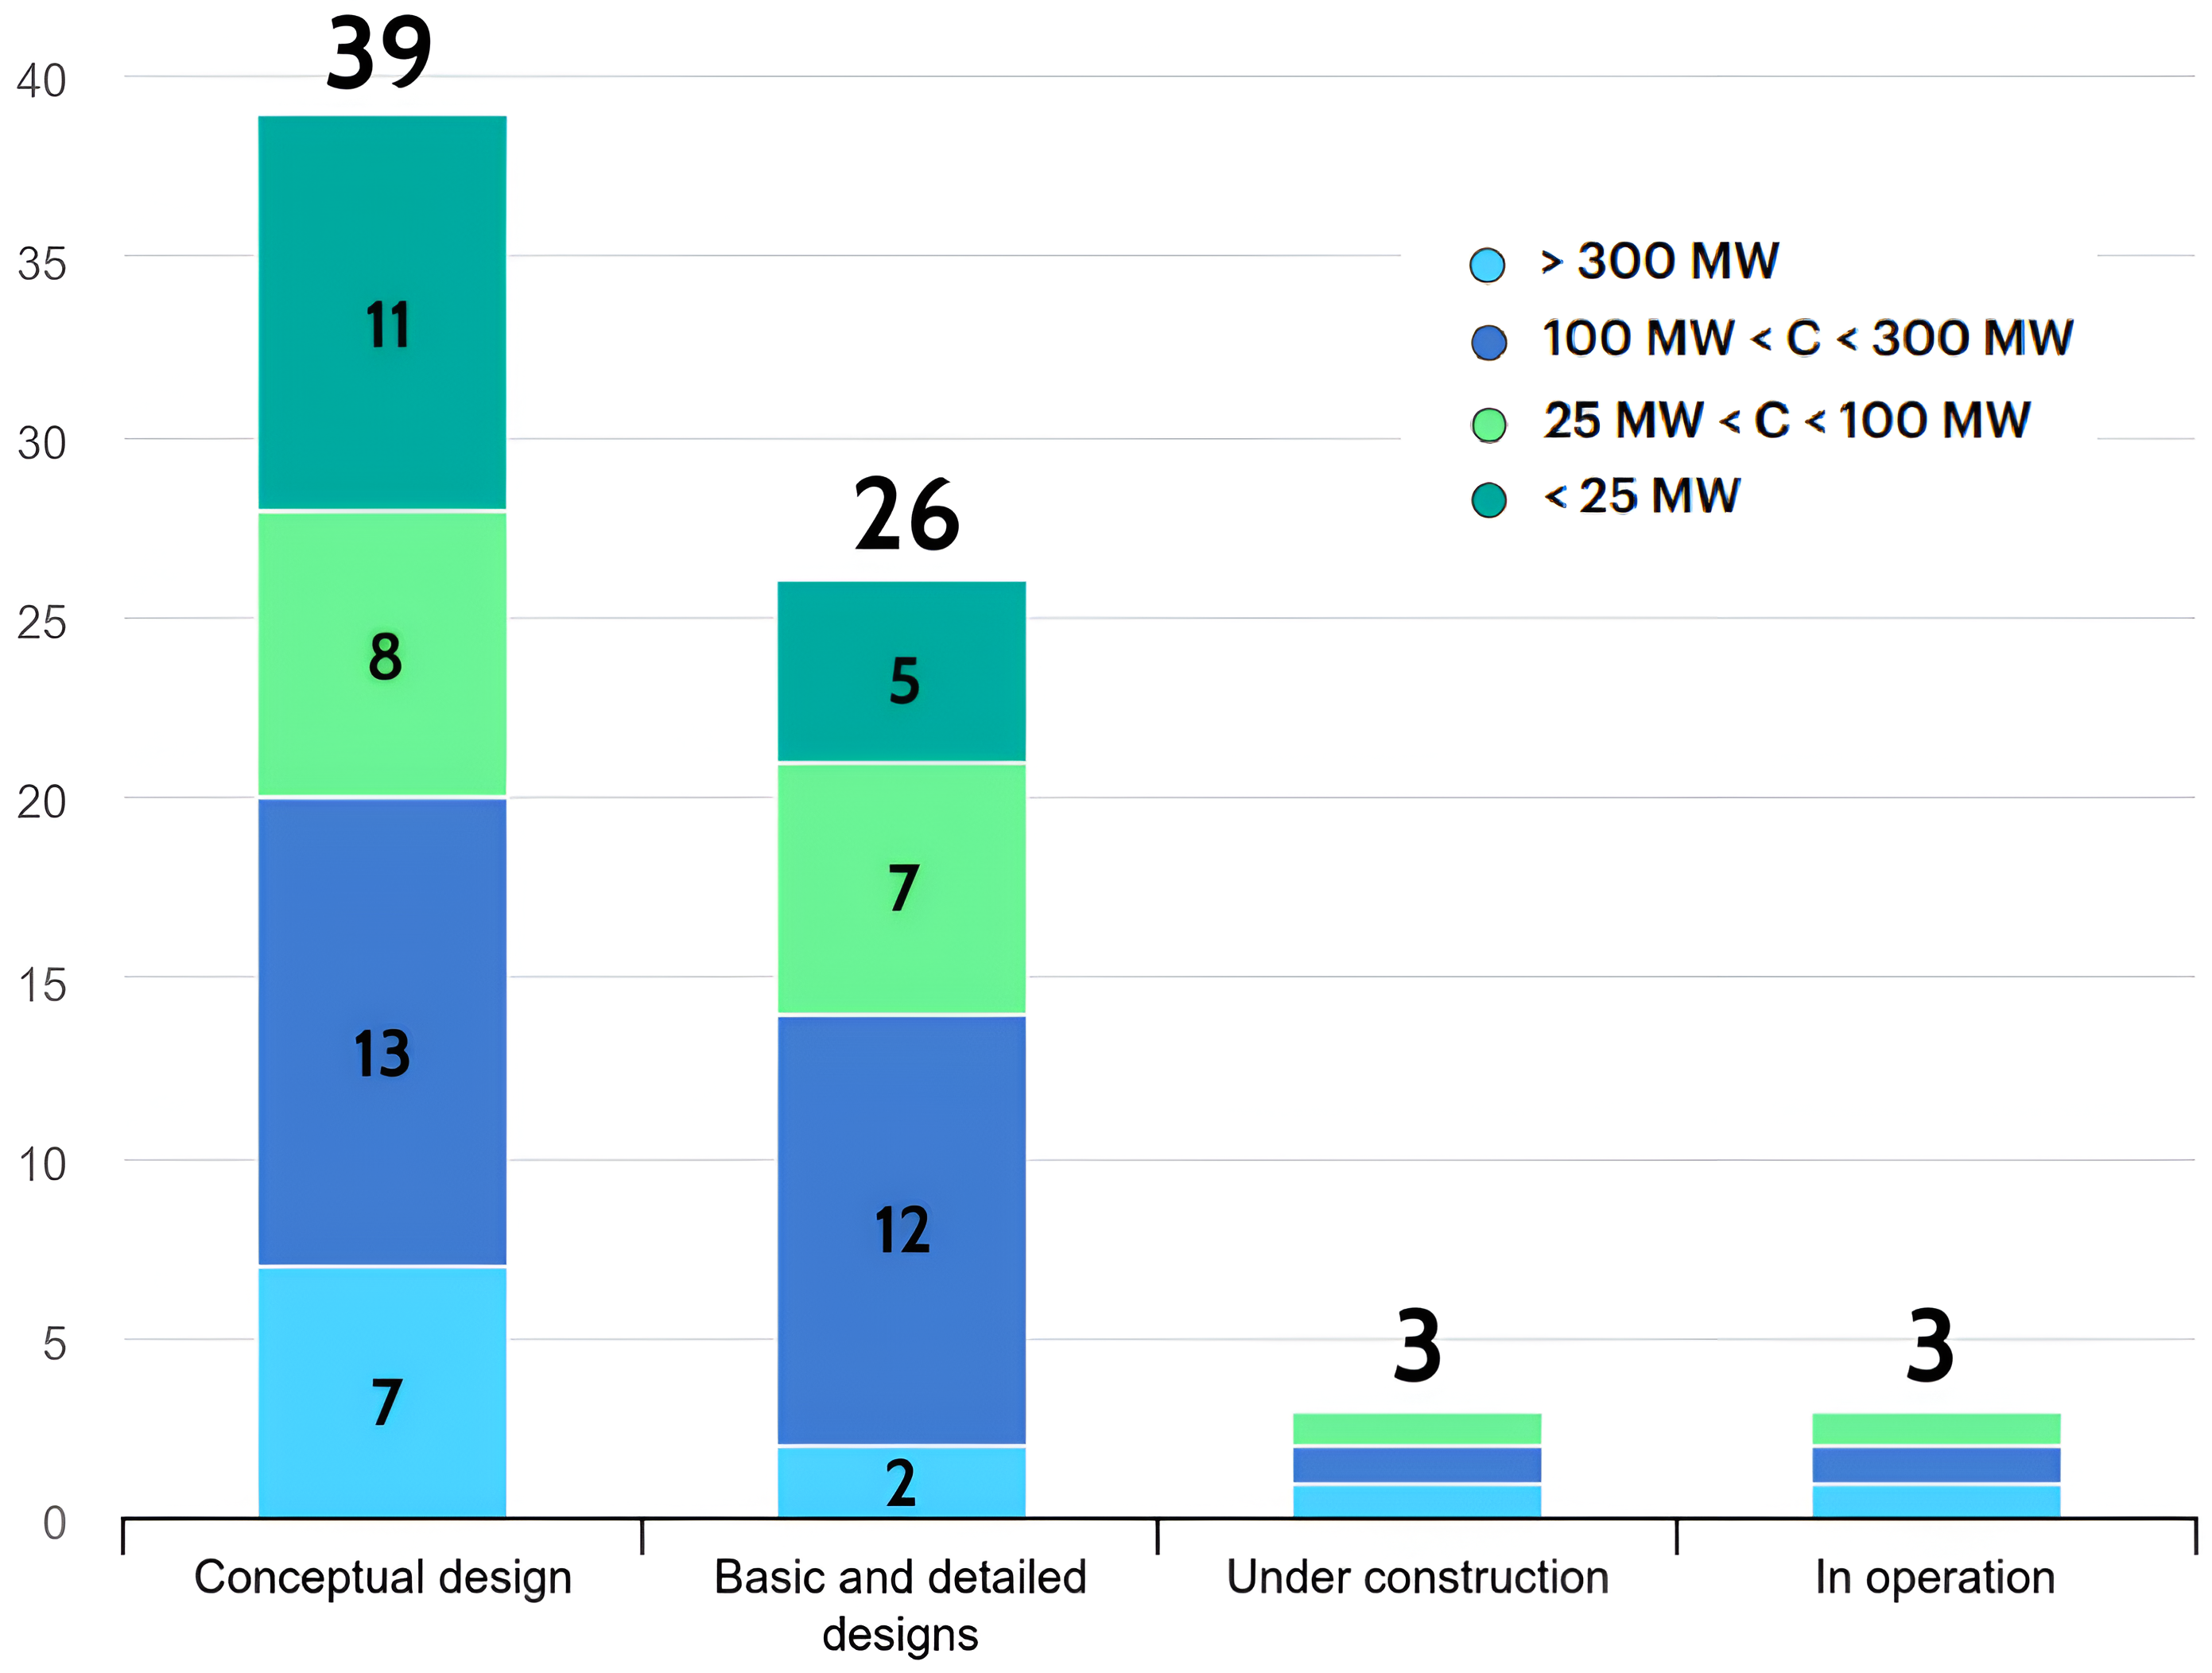
\includegraphics[width=0.52\textwidth]{content/figures/global_smr_projects2.png}
      \caption{\acrshortpl{smr} en el mundo (\cite{iea_global_smr_projects}).}
      \label{fig:global_smr_projects}
      \vspace{-1cm}
    \end{wrapfigure}

    En este contexto, se ha incrementado muy considerablemente el interés por los reactores modulares pequeños, ampliamente conocidos como \emph{\acrfullpl{smr}}. Se trata de una tecnología avanzada de menor escala que la convencional que ofrece grandes ventajas en lo que a coste, tiempo de construcción, seguridad y versatilidad se refiere. Por consiguiente, múltiples instituciones públicas y privadas están participando activamente en los esfuerzos encaminados a hacer prosperar esta tecnología, existiendo más de 80 diseños de \acrshortpl{smr} comerciales que se están desarrollando en todo el mundo (\cite{smr_oiea}).




    
\newpage 

Este creciente empuje de la industria nuclear está contribuyendo a un aumento de profesionales especializados en este sector y, paralelamente, a una creciente necesidad de futuros profesionales nucleares. En este contexto y frente a los grandes avances tecnológicos desarrollados actualmente, cobran una especial importancia los \textbf{simuladores} empleados tanto en el ámbito del análisis numérico como en la formación de operadores, técnicos e ingenieros nucleares. Existen múltiples simuladores virtuales y físicos desarrollados por diversas instituciones y empresas que permiten enfrentarse a las condiciones de operación, maniobras y accidentes que pueden suceder en una central nuclear. La Escuela Técnica Superior de Ingenieros Industriales de Madrid (ETSII - UPM) tiene a su disposición el \acrfull{sgiz}, con el cual se trabajará en el presente proyecto para profundizar en el estudio de la operación de las centrales nucleares y, en concreto, en la operación de un \acrshort{smr}, debido a las grandes similitudes que el simulador en cuestión presenta con respecto a esta innovadora tecnología.

\subsection{Objetivos}

El principal objetivo de este trabajo fin de grado es \textbf{simular maniobras de seguimiento de carga de una central nuclear muy similar a un \acrshort{smr}} mediante el \acrshort{sgiz} de la Escuela. Este tipo de maniobras es una de las aplicaciones fundamentales para las que se concibe el diseño de los \acrshortpl{smr} y presentan un gran interés actualmente. Para ello, y como segundo objetivo fundamental, se pretende \textbf{conocer en profundidad el funcionamiento de un \acrshort{smr}; sus sistemas de seguridad, protección y control, y su modo de operación}.

Asimismo, existen paralelamente diversos objetivos secundarios. En primer lugar, familiarizarse con el tipo de software empleado en los simuladores del ámbito nuclear. En segundo lugar, conocer el estado del arte, las características, las grandes ventajas y los desafíos de la tecnología de los \acrshortpl{smr}. Por último, implementar las simulaciones realizadas al programa de prácticas de la asignatura de Tecnologías Avanzadas en Reactores Nucleares del Máster en Ciencia y Tecnología Nuclear impartido en la ETSII.

\subsection{Metodología}

El desarrollo de este proyecto parte de una adquisición completa de diversos conceptos teóricos que permitirán posteriormente focalizarse en la realización de simulaciones prácticas. Al mismo tiempo, estas simulaciones complementarán y consolidarán los conocimientos previos adquiridos y posibilitarán un aprendizaje en profundidad. De esta manera, el trabajo se fundamenta, en tres grandes bloques:

\begin{itemize}
  \item \textbf{Los \acrlongpl{smr}:} Comenzando por los orígenes de esta tecnología, posteriormente se analizan detalladamente las ventajas que presenta frente a los reactores de gran escala y se clasifican los distintos tipos de pequeños reactores modulares existentes. Por último, se analiza un \acrshort{smr} en concreto ---el AP300--- por su similitud con el reactor del simulador con el que se trabaja ---el \acrshort{sgiz}---.
  \item \textbf{Los simuladores:} En primer lugar, se clasifican los distintos tipos de simuladores existentes en función de los objetivos, las ventajas y las funcionalidades que presentan. En segundo lugar, se analizan casos concretos de simuladores de \acrshortpl{smr} para conocer el estado del arte de este tipo de simulación. Seguidamente, se detallan las ventajas del empleo de simuladores para fines formativos y didácticos. Por último, se estudia la Central Nuclear de Zorita, a la cual pertenece el \acrshort{sgiz}, comparándola con el AP300 para ver su parecido con un \acrshort{smr}. Además, se finaliza este estudio con una descripción de las características y modos de operación del \acrshort{sgiz}.
  \item \textbf{Las simulaciones:} Como el proyecto se centra en el análisis de las capacidades de seguimiento de carga de los \acrshortpl{smr}, se comienza este apartado práctico con un estudio de este tipo de maniobras de variación de potencia en función de distintas necesidades. Seguidamente, se realizan múltiples simulaciones que, tras ser debidamente analizadas, permiten comprender en profundidad, no solo el seguimiento de carga, sino también el funcionamiento y los  sistemas más importantes de una central nuclear. En este bloque se incluye la implementación de una de las simulaciones como práctica académica.
\end{itemize}
\newpage

% Formato APA (el recomendado para TFG)

\appto{\bibsetup}{\sloppy}

\printbibliography[heading=bibintoc, title=BIBLIOGRAFÍA] % Aparecen únicamente las referencias citadas a lo largo del documento
%%%%%%%%%%%%%%%%%%% - ANEXOS - %%%%%%%%%%%%%%%%%%%

\newpage
\section*{ANEXOS} \label{sec:anexos} % Se añade un asterisco a \section para que el título no esté numerado.
\phantomsection
\addcontentsline{toc}{section}{ANEXOS} % Al utilizar \section* se ha de añadir manualmente el apartado al índice (Table Of Contents, TOC).
\markright{ANEXOS} % Al utilizar \section* se ha de añadir manualmente el título del apartado al encabezado.

\renewcommand{\thesubsection}{\Alph{subsection}} % Se numeran los anexos con letras del alfabeto en lugar de números.
% Se indica que las tablas, figuras y códigos se numeran con el código del anexo (A, B, C, ...) seguido del número de tabla, figura o código dentro del anexo (tabla A.2, figura C.1, etc.)
\renewcommand{\thetable}{\Alph{subsection}.\arabic{table}}
\renewcommand{\thefigure}{\Alph{subsection}.\arabic{figure}}
\renewcommand{\thecode}{\Alph{subsection}.\arabic{code}}

% ---------------- Primer anexo ---------------- %
\setcounter{subsection}{0}
\setcounter{table}{0}
\setcounter{figure}{0}

\subsection{Gráficas obtenidas en la segunda simulación larga fallida} \label{graficas_erroneas}

\textit{Simulación de 6 horas y 40 minutos realizada en el \acrshort{sgiz} el 30 de abril de 2024.}

A continuación, se muestran algunas de las gráficas obtenidas en la simulación fallida explicada en el apartado \ref{sim_larga_fallida}, con una estabilización incorrecta a partir de las 4 horas:

\begin{figure}[!h]
    \centering
    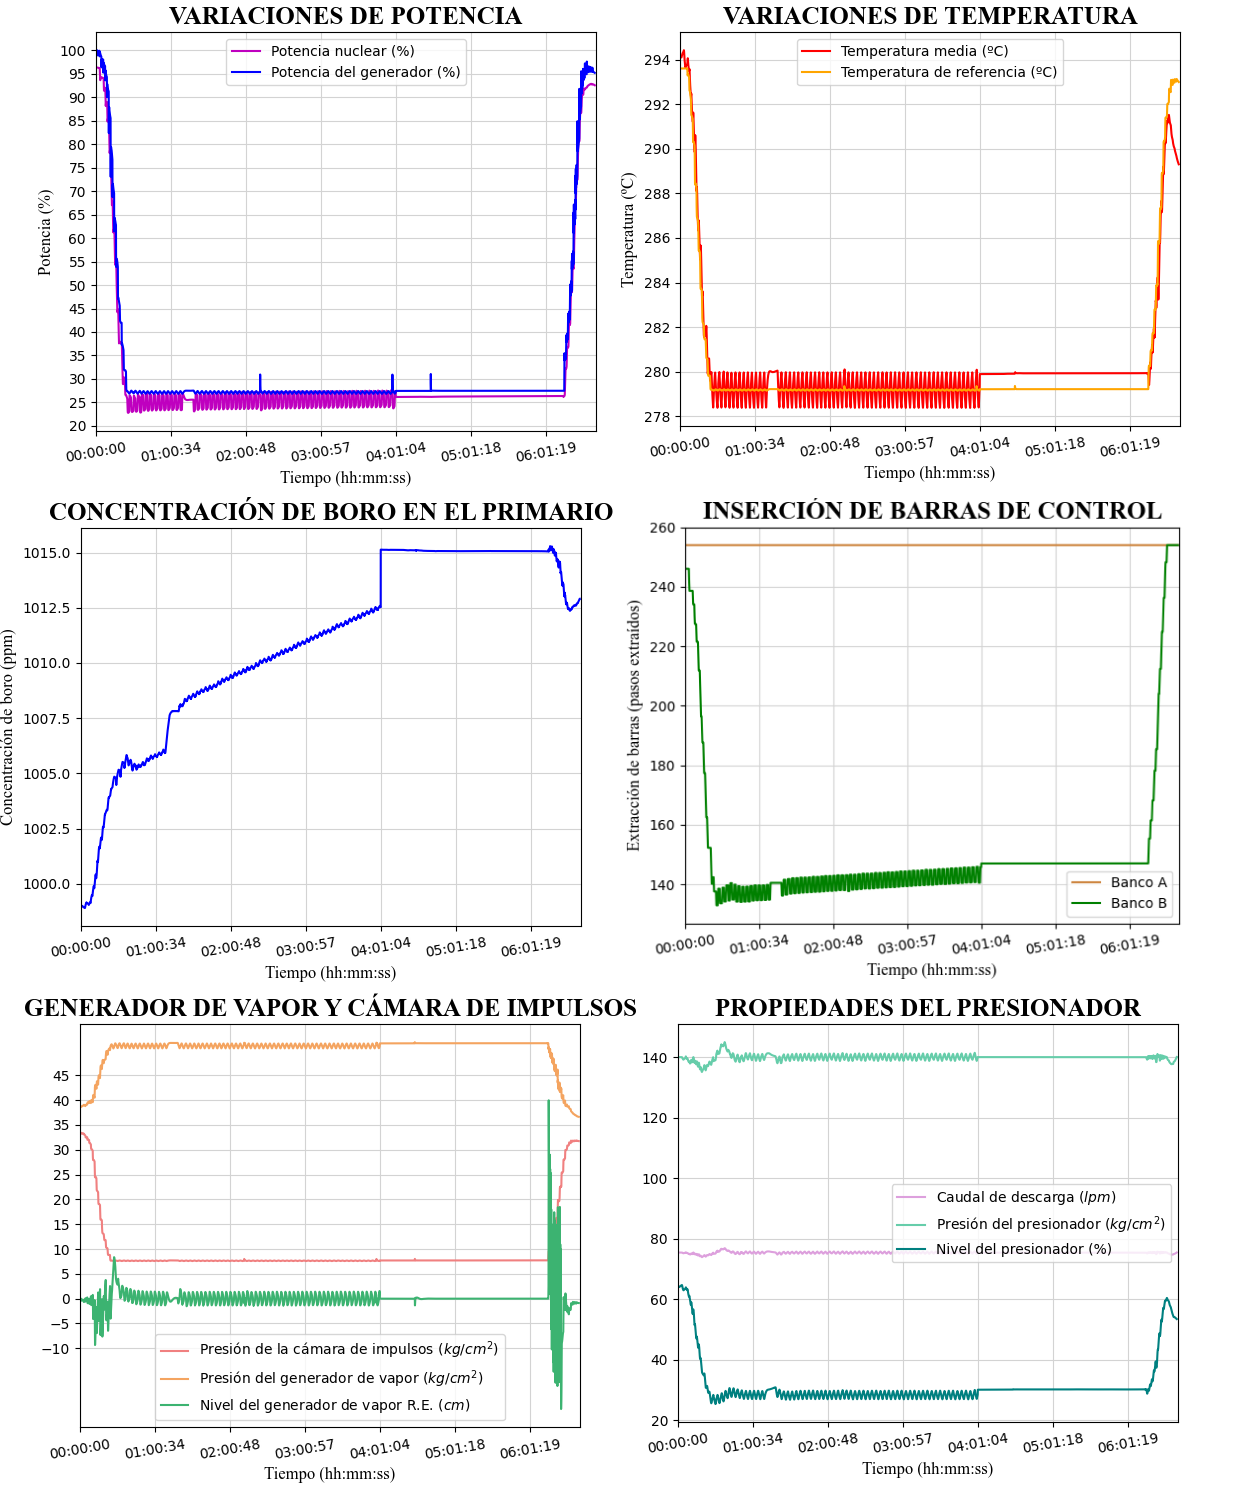
\includegraphics[width=\textwidth]{content/figures/sim2_peque.png}
    \caption{Gráficas imperfectas de la segunda simulación larga fallida.}
    \label{fig:sim2_peque}
\end{figure}

\newpage
\subsection{Resultados de la encuesta de la práctica} \label{resultados_encuesta_practica}

Tal y como se comenta en el apartado \ref{feedback_practica}, tras la realización de la práctica de seguimiento de carga en el \acrshort{sgiz} por parte de 28 alumnos de la asignatura de \textit{Tecnologías Avanzadas en Reactores Nucleares} del máster, se envió una encuesta para obtener retroalimentación sobre la sesión. A continuación, se muestran los resultados detallados de las 12 respuestas obtenidas:

\begin{enumerate}
    \item \textbf{¿Habías hecho alguna práctica similar en el \acrshort{sgiz} anteriormente?}
    
    \begin{figure}[!h]
        \centering
        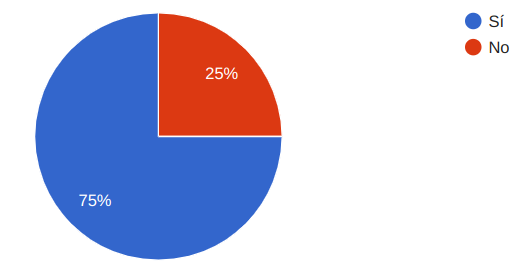
\includegraphics[width=0.47\textwidth]{content/figures/encuesta_1.png}
        \caption{Resultados pregunta 1.}
        \label{fig:encuesta_1}
    \end{figure}

    \item \textbf{¿Crees que la práctica se enmarca adecuadamente en la asignatura de Tecnologías Avanzadas en Reactores Nucleares?}
    
    \begin{figure}[!h]
        \centering
        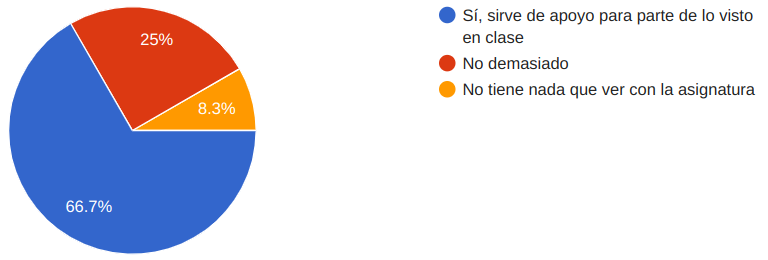
\includegraphics[width=0.72\textwidth]{content/figures/encuesta_2.png}
        \caption{Resultados pregunta 2.}
        \label{fig:encuesta_2}
    \end{figure}
    
    \item \textbf{¿Habías oído hablar antes de las capacidades avanzadas de seguimiento de carga para las que se diseñan los \acrlongpl{smr}?}
    
    \begin{figure}[!h]
        \centering
        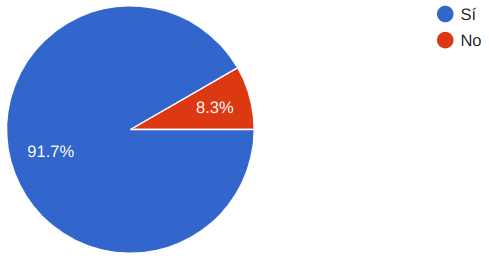
\includegraphics[width=0.47\textwidth]{content/figures/encuesta_3.png}
        \caption{Resultados pregunta 3.}
        \label{fig:encuesta_3}
    \end{figure}
    
    \newpage
    \item \textbf{¿Has aprendido cosas nuevas con la práctica?}
    \newline
    \begin{figure}[h]
        \centering
        \vspace{-0.5cm}
        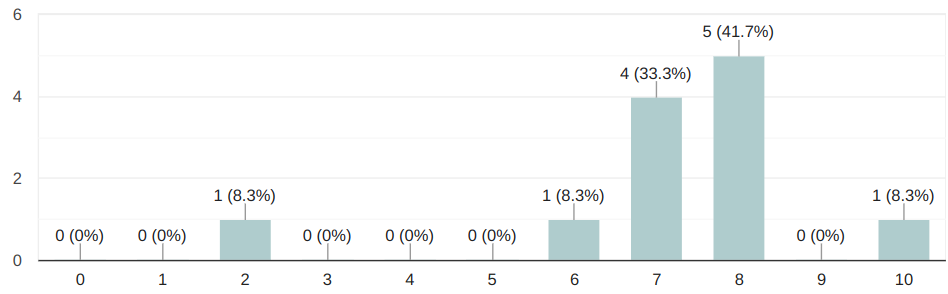
\includegraphics[width=\textwidth]{content/figures/encuesta_4.png}
        \caption{Resultados pregunta 4.}
        \label{fig:encuesta_4}
    \end{figure}
    
    \item \textbf{¿Te ha ayudado a comprender mejor las características y el funcionamiento general de los principales componentes y sistemas del reactor durante la operación del mismo?}
    
    \begin{figure}[h]
        \centering
        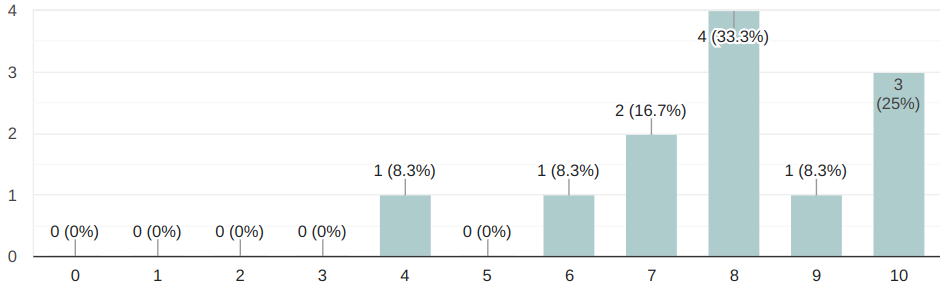
\includegraphics[width=\textwidth]{content/figures/encuesta_5.png}
        \caption{Resultados pregunta 5.}
        \label{fig:encuesta_5}
    \end{figure}
    
    \item \textbf{¿Se han entendido bien el objetivo, el procedimiento y las conclusiones de la simulación realizada? ¿Las explicaciones han sido suficientemente claras?}
    
    \begin{figure}[!h]
        \centering
        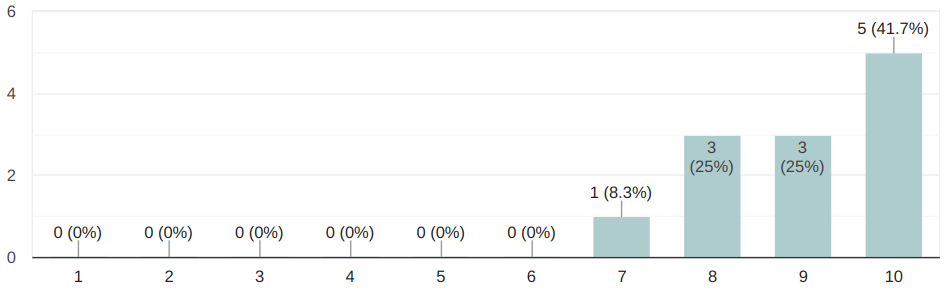
\includegraphics[width=\textwidth]{content/figures/encuesta_6.png}
        \caption{Resultados pregunta 6.}
        \label{fig:encuesta_6}
    \end{figure}
    
    \newpage
    \item \textbf{En general, ¿crees que realizar prácticas en el simulador ayuda a entender mejor lo visto en algunas asignaturas del grado y del máster?}
    
    \begin{figure}[!h]
        \centering
        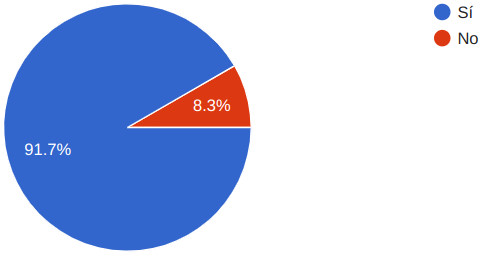
\includegraphics[width=0.47\textwidth]{content/figures/encuesta_7.png}
        \caption{Resultados pregunta 7.}
        \label{fig:encuesta_7}
    \end{figure}

    \item \textbf{Finalmente, valora del 0 al 10 tu grado de satisfacción general con la práctica realizada:}
    
    \begin{figure}[!h]
        \centering
        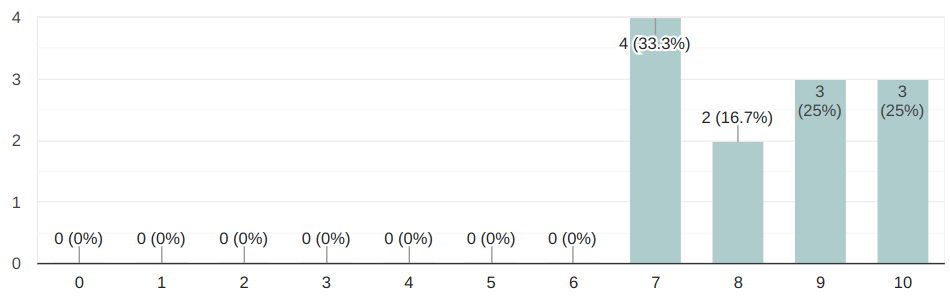
\includegraphics[width=\textwidth]{content/figures/encuesta_8.png}
        \caption{Resultados pregunta 8.}
        \label{fig:encuesta_8}
    \end{figure}
\end{enumerate}

Además de las 8 preguntas mostradas, se añadió una sección en el formulario para que los alumnos hicieran comentarios adicionales. La información aportada en esa sección es de gran utilidad y se encuentra resumida en el apartado \ref{feedback_practica}.

\newpage
\subsection{Código} \label{sec:codigo}

Todas las gráficas de las simulaciones realizadas en el \acrshort{sgiz} han sido elaboradas con \textit{Python} a partir de los datos generados en \textit{Excel} por el propio simulador. A continuación, se muestra, a modo de ejemplo, el código para la obtención de una de las gráficas:

\vspace{-5pt}

\begin{code}[H]
\begin{lstlisting}[firstnumber=1, breakindent=55pt]
  # Importación de las librerías necesarias
  import matplotlib.pyplot as plt
  import numpy as np
  import pandas as pd

  # Obtención de datos:
  gen_vapor_camara_imp=pd.read_excel("simulacion3.xlsx","gen_vapor_camara_imp")
  df_gen_vapor_camara_imp=pd.DataFrame=gen_vapor_camara_imp

  tiempo=[]
  for i in range(0,len(df_gen_vapor_camara_imp.tiempo)):
      tiempo.append(df_gen_vapor_camara_imp.tiempo[i].strftime('%H:%M:%S'))
    
  pres_cam_imp=[]
  for i in range(0,len(df_gen_vapor_camara_imp.pres_cam_imp)):
      pres_cam_imp.append(df_gen_vapor_camara_imp.pres_cam_imp[i])

  presion_gen_vapor=[]
  for i in range(0,len(df_gen_vapor_camara_imp.               presion_gen_vapor)):
      presion_gen_vapor.append(df_gen_vapor_camara_imp.presion_gen_vapor[i])

  nivel_gen_vapor=[]
  for i in range(0,len(df_gen_vapor_camara_imp.nivel_gen_vapor)):
      nivel_gen_vapor.append(df_gen_vapor_camara_imp.nivel_gen_vapor[i])

  # Creación del gráfico
  plt.plot(tiempo, presion_camara_impulsos, label='Presión de la cámara de impulsos $(kg/cm^2)$', color='lightcoral')
  plt.plot(tiempo, presion_gen_vapor, label='Presión del generador de vapor $(kg/cm^2)$', color='sandybrown')
  plt.plot(tiempo, nivel_gen_vapor, label='Nivel del generador de vapor R.E. $(cm)$', color='mediumseagreen')

  # Creación de la leyenda y el título
  plt.legend(loc='best')
  plt.xlabel('Tiempo (hh:mm:ss)', family='Times New Roman', size=12)
  plt.title('COMPORTAMIENTO GENERADOR DE VAPOR Y CÁMARA DE IMPULSOS', fontname='Times New Roman', size=18, weight='bold')
  plt.grid(True, color='lightgrey')
  plt.yticks(np.arange(-10,50,5))
  plt.xlim([0, len(tiempo)])
  plt.xticks(np.arange(0,len(tiempo),360))
  plt.xticks(rotation = 10)

  # Mostrar el gráfico
  plt.show()
\end{lstlisting}
\vspace{-5pt}
\caption{Ejemplo del código utilizado para generar las gráficas de las simulaciones. Este en concreto corresponde al código de la figura \ref{fig:sim3_gen_vapor_camara_imp}.}
\label{cod:codigo_graficas}
\end{code}


%%%%%%%%%%%%%% - ÍNDICE DE TABLAS - %%%%%%%%%%%%%%

\newpage

\renewcommand{\listtablename}{ÍNDICE DE TABLAS} % Se define el nombre del índice de tablas.
\listoftables % Se genera automáticamente el índice con las distintas tablas del documento (entorno \table o \longtable).
\addcontentsline{toc}{section}{ÍNDICE DE TABLAS} % Se añade manualmente el apartado al índice (Table Of Contents, TOC).


%%%%%%%%%%%%% - ÍNDICE DE FIGURAS - %%%%%%%%%%%%%%

\newpage

\renewcommand{\listfigurename}{ÍNDICE DE FIGURAS} % Se define el nombre del índice de figuras.
\listoffigures % Se genera automáticamente el índice con las distintas figuras del documento (entorno \figure).
\addcontentsline{toc}{section}{ÍNDICE DE FIGURAS} % Se añade manualmente el apartado al índice (Table Of Contents, TOC).


%%%%%%%%%%%%%% - FIN DEL DOCUMENTO - %%%%%%%%%%%%%

\end{document}